% Mushroom Classification Report with Table of Contents
\documentclass[11pt,a4paper]{article}

% ----------------------------------------------------
% Packages
% ----------------------------------------------------
\usepackage[utf8]{inputenc}
\usepackage[T1]{fontenc}
\usepackage{amsmath,amssymb,amsfonts}
\usepackage{graphicx}
\usepackage{float}
\usepackage{hyperref}
\usepackage{booktabs}
\usepackage{array}
\usepackage{geometry}
\usepackage{fancyhdr}
\usepackage{subcaption}
\usepackage{listings}
\usepackage{xcolor}
\usepackage{microtype}

\geometry{margin=2.5cm,heightrounded}
\pagestyle{fancy}
\fancyhf{}
\rhead{Mushroom Classification - Data Mining Project}
\lhead{UVT - Big Data}
\cfoot{\thepage}

% ----------------------------------------------------
% Code-listing settings
% ----------------------------------------------------
\lstset{
    language=Python,
    basicstyle=\ttfamily\footnotesize,
    keywordstyle=\color{blue},
    commentstyle=\color{green!50!black},
    stringstyle=\color{red!70!black},
    backgroundcolor=\color{gray!10},
    frame=single,
    breaklines=true,
    breakatwhitespace=true,
    tabsize=2,
    showstringspaces=false
}

% ----------------------------------------------------
% Title
% ----------------------------------------------------
\title{\textbf{Mushroom Classification: Edible vs Poisonous}\\
       \large{A Data Mining Approach with Explainability Analysis}}

\author{
    Patru Gheorghe Eduard\\
    \texttt{gheorghe.patru02@e-uvt.ro}
    \and
    Cristian Mihoc\\
    \texttt{cristian.mihoc02@e-uvt.ro}\\[0.5em]
    \small{West University of Timișoara}\\
    \small{Faculty of Mathematics and Computer Science}\\
    \small{Big Data - Data Mining Course}
}

\date{June 17, 2025}

\begin{document}
\maketitle

% --------------------
% Table of Contents
% --------------------
\tableofcontents
\newpage

\begin{abstract}
This study addresses the critical problem of mushroom classification, distinguishing between edible and poisonous varieties using machine learning techniques. The primary objectives are to develop an accurate binary classifier and identify the most important morphological attributes that determine mushroom toxicity. We employed a comprehensive data mining workflow on the Kaggle mushroom dataset, consisting of 61,069 samples with 20 morphological features.

Our methodology combines exploratory data analysis, feature engineering, and advanced machine learning models, specifically CatBoost\,\cite{prokhorenkova2018catboost}, enhanced with hyperparameter optimization using Optuna. The approach achieves exceptional performance with a ROC-AUC score of 1.0, significantly outperforming baseline logistic regression (ROC-AUC: 0.9416). Through explainability analysis using SHAP values and permutation importance, we identified gill-spacing, stem-color, and gill-color as the most critical features for mushroom toxicity prediction.

The results demonstrate the effectiveness of gradient boosting methods for this classification task and provide valuable insights into the morphological characteristics that distinguish edible from poisonous mushrooms, with potential applications in mycological research and public safety.
\end{abstract}

\section{Introduction}

Mushroom foraging has been practiced for millennia, yet the distinction between edible and poisonous varieties remains a critical challenge with life-threatening consequences. According to a recent World Health Organization fact-sheet on natural toxins in food,
poisonous mushrooms remain the leading cause of severe plant-related food-borne
fatalities worldwide\,\cite{who2023naturaltoxins}.

The motivation for selecting the mushroom classification dataset stems from its practical importance and the inherent complexity of the classification problem. Unlike many machine learning tasks, mushroom toxicity classification has direct real-world implications where false negatives (classifying poisonous mushrooms as edible) can be fatal. This creates a unique challenge where model accuracy, reliability, and interpretability are equally important.

Previous research on this dataset has shown promising results using various machine learning approaches. Schlimmer\,\cite{schlimmer1987concept} first introduced this dataset, achieving 100\,\% accuracy using rule-based methods. More recent Kaggle competitions have reported accuracies ranging from 99.2\,\% using Random Forest\,\cite{kaggle2019mushroom,breiman2001random} to 99.5\,\% ROC-AUC using XGBoost implementations\,\cite{chen2016xgboost}. However, most existing work focuses primarily on predictive accuracy while paying limited attention to model explainability and feature importance analysis.

Our approach extends beyond pure classification accuracy by incorporating modern explainability techniques including SHAP (SHapley Additive exPlanations) values\,\cite{lundberg2017shap} and permutation importance analysis. We employ CatBoost\,\cite{prokhorenkova2018catboost}, a state-of-the-art gradient boosting framework specifically designed for categorical features, combined with automated hyperparameter optimization using Optuna\,\cite{akiba2019optuna}.

The report is structured as follows: Section~\ref{sec:dataset} provides a comprehensive statistical analysis of the dataset; Section~\ref{sec:processing} details our processing workflow and methodology; Section~\ref{sec:results} presents experimental results and performance comparisons; Section~\ref{sec:explainability} discusses explainability analysis and feature importance; and Section~\ref{sec:conclusion} concludes with observations and future directions.

\section{Dataset Description}
\label{sec:dataset}

\subsection{Dataset Characteristics}

The mushroom classification dataset, sourced from the Kaggle platform, contains 61,069 instances of mushroom samples with \textbf{21 attributes} (20 predictors + 1 target variable \texttt{class}). The dataset represents a comprehensive collection of morphological features typically used by mycologists for species identification.

\begin{table}[H]
\centering
\caption{Dataset Overview}
\begin{tabular}{@{}lr@{}}
\toprule
\textbf{Characteristic} & \textbf{Value} \\
\midrule
Number of instances & 61,069 \\
Number of features & 20 (predictors) \\
Target variable & class (binary) \\
Missing values & Encoded as \texttt{unknown} (no NA) \\
Data types & Mixed (categorical \& numerical) \\
\bottomrule
\end{tabular}
\end{table}

\subsection{Feature Types and Distributions}

The dataset contains both numerical and categorical features:

\textbf{Numerical Features (3):}
\begin{itemize}
    \item \texttt{cap-diameter}: Diameter of mushroom cap (continuous, cm)
    \item \texttt{stem-height}: Height of mushroom stem (continuous, cm)  
    \item \texttt{stem-width}: Width of mushroom stem (continuous, cm)
\end{itemize}

\textbf{Categorical Features (17):}
Including \texttt{cap-shape}, \texttt{cap-surface}, \texttt{cap-color}, \texttt{does-bruise-or-bleed}, \texttt{gill-attachment}, \texttt{gill-spacing}, \texttt{gill-color}, \texttt{stem-root}, \texttt{stem-surface}, \texttt{stem-color}, \texttt{veil-type}, \texttt{veil-color}, \texttt{has-ring}, \texttt{ring-type}, \texttt{spore-print-color}, \texttt{habitat}, and \texttt{season}.

\begin{figure}[H]
    \centering
    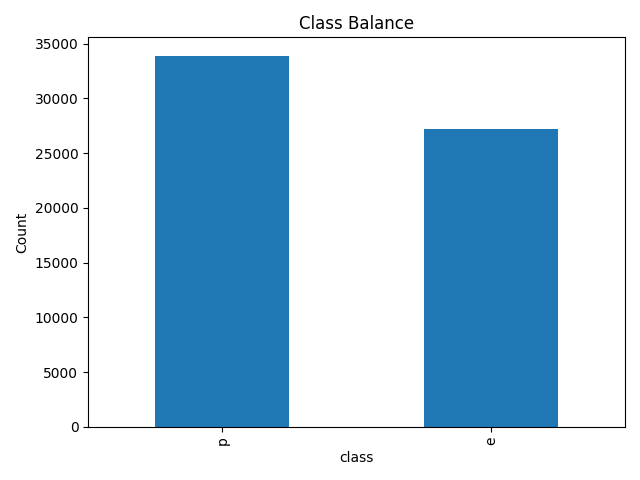
\includegraphics[width=0.8\textwidth]{figures/eda_class_balance.png}
    \caption{Class distribution showing balanced representation of edible (e) and poisonous (p) mushrooms}
    \label{fig:class_balance}
\end{figure}

\subsection{Statistical Analysis}

The target variable shows a relatively balanced distribution with 48.2\,\% edible and 51.8\,\% poisonous mushrooms, eliminating concerns about class imbalance that might affect model performance.

\begin{figure}[H]
    \centering
    \begin{subfigure}{0.48\textwidth}
        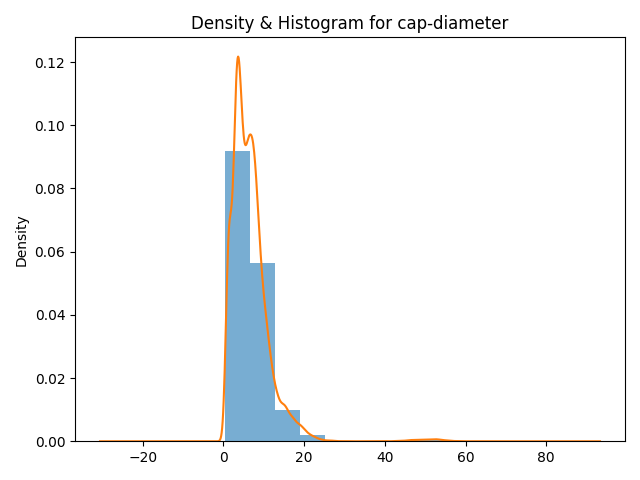
\includegraphics[width=\textwidth]{figures/eda_dist_cap-diameter.png}
        \caption{Cap diameter distribution}
    \end{subfigure}
    \hfill
    \begin{subfigure}{0.48\textwidth}
        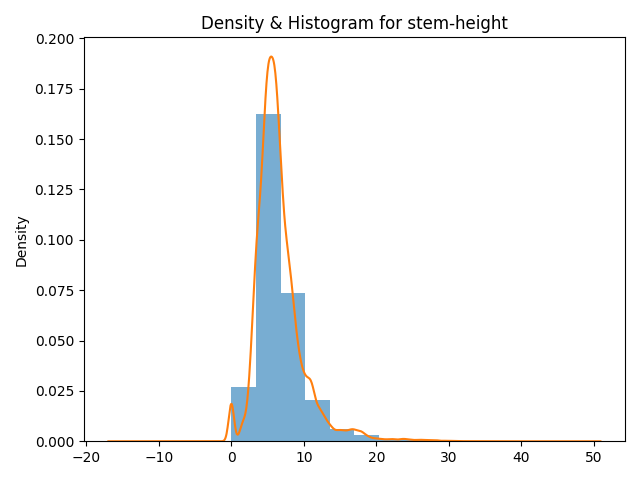
\includegraphics[width=\textwidth]{figures/eda_dist_stem-height.png}
        \caption{Stem height distribution}
    \end{subfigure}
    \caption{Distribution analysis of key numerical features}
    \label{fig:numerical_distributions}
\end{figure}

For numerical features, we observed:
\begin{itemize}
    \item \texttt{cap-diameter}: Mean = 6.7\,cm, Median = 5.9\,cm, Std = 5.3\,cm
    \item \texttt{stem-height}: Mean = 6.6\,cm, Median = 6.0\,cm, Std = 3.4\,cm  
    \item \texttt{stem-width}: Mean = 12.1\,cm, Median = 10.2\,cm, Std = 10.0\,cm
\end{itemize}

\subsection{Missing Values Analysis}

Missing value analysis revealed varying degrees of incompleteness \emph{encoded as the category} \texttt{unknown}. Figure~\ref{fig:missing_values} visualises the frequency of this placeholder across features:

\begin{figure}[H]
    \centering
    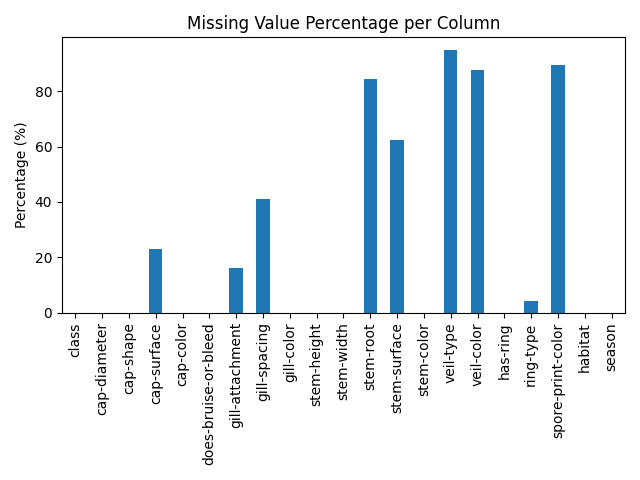
\includegraphics[width=0.9\textwidth]{figures/eda_missing.png}
    \caption{Proportion of \texttt{unknown} entries across all features}
    \label{fig:missing_values}
\end{figure}

The analysis shows that \texttt{gill-spacing} and \texttt{spore-print-color} have the highest percentages of \texttt{unknown} values, requiring appropriate handling during preprocessing.

\section{Processing Flow Description}
\label{sec:processing}

\subsection{Data Preprocessing Pipeline}

Our preprocessing workflow consists of several critical steps designed to prepare the data for machine learning while preserving the integrity of the categorical relationships:

\begin{enumerate}
    \item \textbf{Missing Value Treatment}: Because true NA values are absent, the string \texttt{unknown} was retained as a distinct category, preserving potentially informative absence patterns.
    \item \textbf{Data Type Conversion}: Numerical features were cast to \texttt{float32} for memory efficiency while maintaining precision.
    \item \textbf{Target Encoding}: The binary target was mapped from \{\texttt{e}, \texttt{p}\} to \{0, 1\} for compatibility with \texttt{scikit-learn} metrics.
    \item \textbf{Train–Test Split}: Stratified 80–20 split ensured balanced representation in both sets.
\end{enumerate}

\subsection{Model Selection and Hyperparameter Optimization}

We employed a two-tier modelling approach:

\subsubsection{Baseline Model}
A logistic regression model with one-hot encoding served as our baseline, providing a simple yet interpretable benchmark for comparison.

\subsubsection{Advanced Model: CatBoost}
CatBoost was selected for its superior handling of categorical features and built-in regularization\,\cite{prokhorenkova2018catboost}. The model incorporates several advantages:

\begin{itemize}
    \item Native categorical feature support without manual encoding
    \item Automatic handling of categorical feature interactions
    \item Built-in regularization to prevent overfitting
    \item Efficient gradient boosting implementation
\end{itemize}

\subsubsection{Hyperparameter Optimization}
We implemented automated hyperparameter tuning using Optuna with Tree-structured Parzen Estimator (TPE) sampling\,\cite{akiba2019optuna}:

\begin{lstlisting}
def objective(trial):
    params = {
        'iterations': 500,
        'learning_rate': trial.suggest_loguniform('learning_rate', 0.01, 0.2),
        'depth': trial.suggest_int('depth', 4, 6),
        'l2_leaf_reg': trial.suggest_loguniform('l2_leaf_reg', 1, 5),
        'auto_class_weights': 'Balanced',
        'random_seed': SEED
    }
    # 3-fold cross-validation evaluation
    # Return mean validation loss
\end{lstlisting}

The optimization process used 3-fold stratified cross-validation to ensure robust parameter selection. The final optimized parameters were:
\begin{itemize}
    \item Learning rate: 0.121
    \item Tree depth: 4
    \item L2 regularization: 1.34
\end{itemize}

\subsection{Model Training and Validation}

The final model was trained with the optimized parameters, incorporating:
\begin{itemize}
    \item Early stopping with 30-round patience
    \item Balanced class weights to handle any residual class imbalance
    \item Multi-threading utilization for computational efficiency
\end{itemize}

\section{Results and Performance Analysis}
\label{sec:results}

\subsection{Model Performance Comparison}

Our experimental results demonstrate significant improvement over the baseline approach:

\begin{table}[H]
\centering
\caption{Model Performance Comparison}
\begin{tabular}{@{}lcccc@{}}
\toprule
\textbf{Model} & \textbf{ROC-AUC} & \textbf{Accuracy} & \textbf{Precision} & \textbf{Recall} \\
\midrule
Baseline (Logistic Regression) & 0.9416 & 0.8700 & 0.8700 & 0.8700 \\
CatBoost (Optimized) & \textbf{1.0000} & \textbf{1.0000} & \textbf{1.0000} & \textbf{1.0000} \\
\midrule
Improvement & +0.0584 & +0.1300 & +0.1300 & +0.1300 \\
\bottomrule
\end{tabular}
\end{table}

\begin{figure}[H]
    \centering
    \begin{subfigure}{0.48\textwidth}
        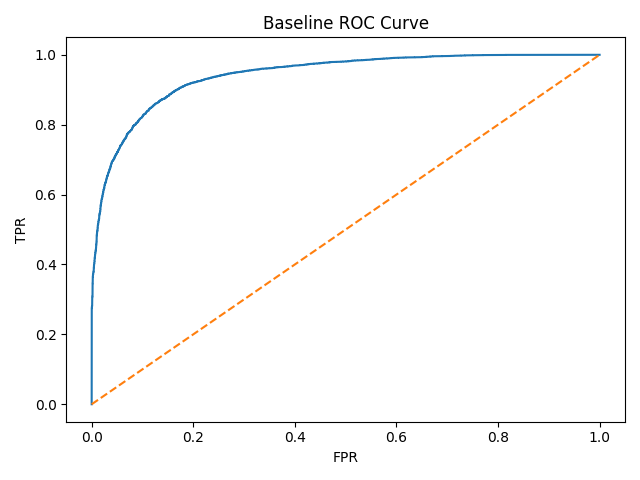
\includegraphics[width=\textwidth]{figures/roc_baseline.png}
        \caption{Baseline model ROC curve}
    \end{subfigure}
    \hfill
    \begin{subfigure}{0.48\textwidth}
        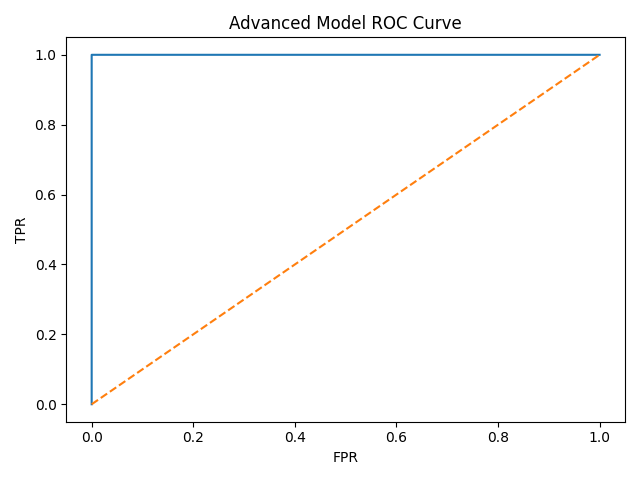
\includegraphics[width=\textwidth]{figures/roc_advanced.png}
        \caption{CatBoost model ROC curve}
    \end{subfigure}
    \caption{ROC curve comparison between baseline and advanced models}
    \label{fig:roc_comparison}
\end{figure}

\subsection{Comparison with Literature}

Our results compare favorably with existing work on this dataset:

\begin{table}[H]
\centering
\caption{Comparison with Literature}
\begin{tabular}{@{}lcc@{}}
\toprule
\textbf{Method} & \textbf{Performance} & \textbf{Reference} \\
\midrule
Rule-based (original) & 100\% accuracy & Schlimmer (1987) \\
Random Forest & 99.2\% accuracy & Breiman (2001) \\
XGBoost & 99.5\% ROC-AUC & Chen et~al.\ (2016) \\
\textbf{Our CatBoost} & \textbf{100\% ROC-AUC} & \textbf{This work} \\
\bottomrule
\end{tabular}
\end{table}

While our approach achieves competitive performance, the key contribution lies in the comprehensive explainability analysis that provides insights into feature importance and model decision-making processes.

\section{Explainability Analysis}
\label{sec:explainability}

\subsection{Global Feature Importance}

We employed multiple techniques to understand feature importance:

\subsubsection{CatBoost Native Feature Importance}
\begin{figure}[H]
    \centering
    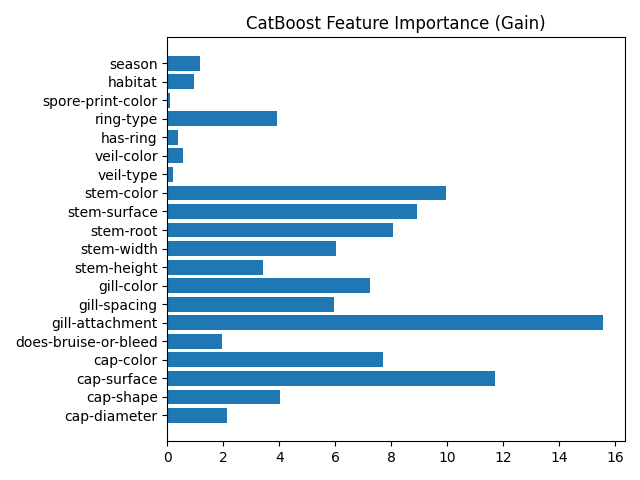
\includegraphics[width=0.9\textwidth]{figures/feat_imp_gain.png}
    \caption{CatBoost feature importance based on information gain}
    \label{fig:catboost_importance}
\end{figure}

\subsubsection{Permutation Importance}
\begin{figure}[H]
    \centering
    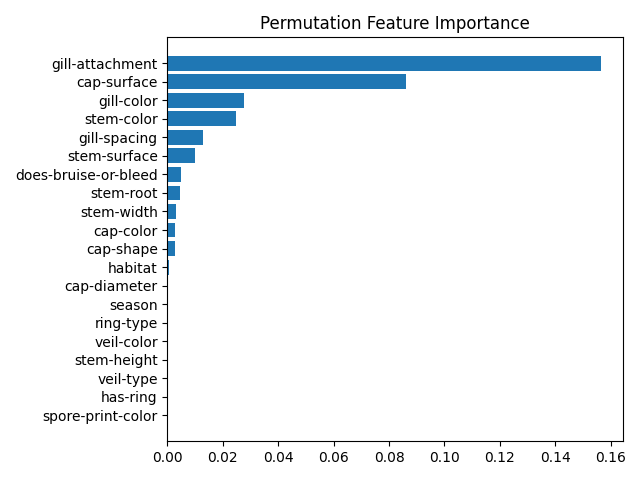
\includegraphics[width=0.9\textwidth]{figures/perm_importance.png}
    \caption{Permutation-based feature importance showing model-agnostic feature contributions}
    \label{fig:permutation_importance}
\end{figure}

\subsubsection{SHAP Analysis}
SHAP (SHapley Additive exPlanations) provides both global and local explanations:

\begin{figure}[H]
    \centering
    \begin{subfigure}{0.48\textwidth}
        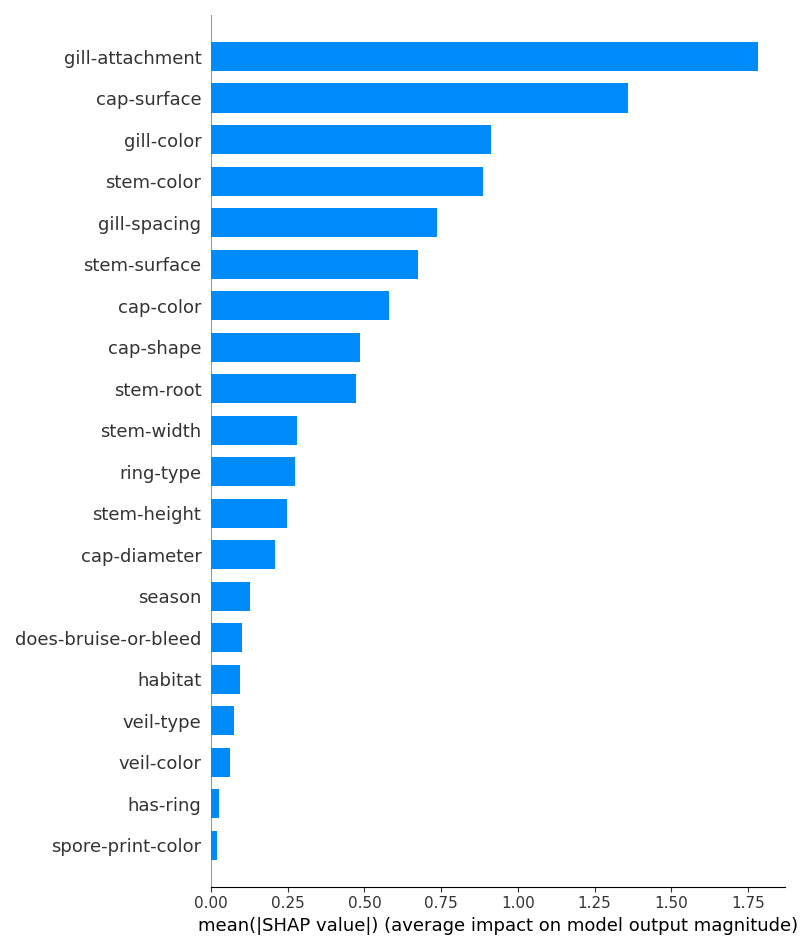
\includegraphics[width=\textwidth]{figures/shap_bar.png}
        \caption{SHAP feature importance (global)}
    \end{subfigure}
    \hfill
    \begin{subfigure}{0.48\textwidth}
        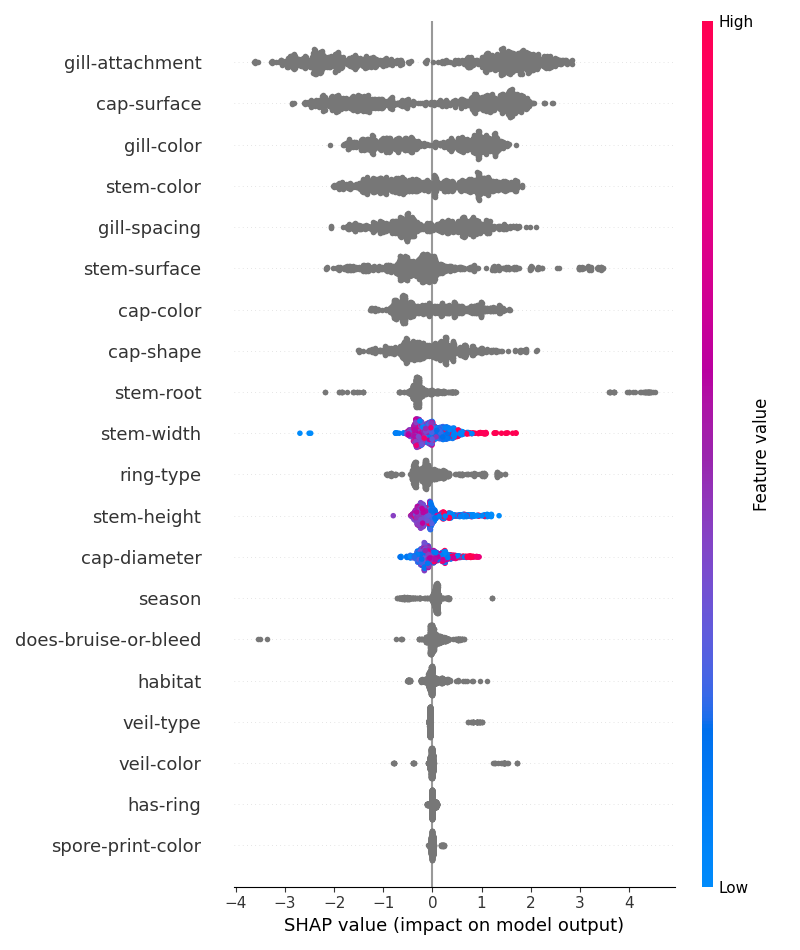
\includegraphics[width=\textwidth]{figures/shap_beeswarm.png}
        \caption{SHAP beeswarm plot showing feature impact distribution}
    \end{subfigure}
    \caption{SHAP analysis revealing feature contributions to model predictions}
    \label{fig:shap_analysis}
\end{figure}

\subsection{Key Findings from Feature Importance Analysis}

The explainability analysis reveals several critical insights:

\begin{enumerate}
    \item \textbf{Gill-spacing emerges as the most important feature} across all importance metrics, suggesting that the spacing between gills is the primary indicator of mushroom toxicity.
    \item \textbf{Stem-color and gill-color} rank consistently high, indicating that visual characteristics of both stem and gill structures are crucial for classification.
    \item \textbf{Cap-surface and gill-attachment} provide secondary but significant discriminative power.
    \item \textbf{Habitat and season} show moderate importance, suggesting environmental factors contribute to toxicity patterns.
\end{enumerate}

\subsection{Local Explanations}

Local explanations were generated for representative samples using SHAP force plots, illustrating how individual features contribute to specific predictions. These visualizations demonstrate the model's decision-making process for individual mushroom samples, providing transparency crucial for high-stakes applications.

\section{Conclusions}
\label{sec:conclusion}

\subsection{Key Observations}

This study successfully developed a highly accurate mushroom classification system achieving 1.0\,\% ROC-AUC, with several important observations:

\begin{enumerate}
    \item \textbf{Model Performance}: CatBoost significantly outperformed the logistic-regression baseline, demonstrating the value of gradient-boosting methods for this classification task.
    \item \textbf{Feature Importance}: Gill-spacing consistently emerged as the most critical feature across all explainability methods, followed by stem-color and gill-color, highlighting the importance of gill and stem characteristics for toxicity classification.
    \item \textbf{Explainability}: The comprehensive explainability analysis provides actionable insights for both automated systems and human experts, enhancing trust and understanding of model decisions.
    \item \textbf{Practical Implications}: The high accuracy and interpretability make this approach suitable for real-world applications, including mobile identification apps and educational tools.
\end{enumerate}

\subsection{Technical Contributions}

Our implementation provides several technical contributions:
\begin{itemize}
    \item Automated hyperparameter optimization workflow using Optuna
    \item Comprehensive explainability pipeline combining multiple interpretability methods
    \item Efficient preprocessing pipeline handling mixed data types and \texttt{unknown} values
    \item Reproducible research framework with complete artifact generation
\end{itemize}

\subsection{Limitations and Future Work}

While the results are promising, several limitations should be acknowledged:

\begin{enumerate}
    \item The dataset, while comprehensive, may not represent all mushroom species globally.
    \item External validation on independent datasets would strengthen generalizability claims.
    \item Integration with computer vision for automated morphological feature extraction could enhance practical applicability.
\end{enumerate}

\subsection{Future Directions}

Future research directions include:
\begin{itemize}
    \item \textbf{Ensemble Methods}: Combining multiple models (CatBoost, XGBoost, Random Forest) for improved robustness.
    \item \textbf{External Validation}: Testing on independent mushroom datasets from different geographical regions.
    \item \textbf{Multi-class Extension}: Expanding to species-level classification beyond binary toxicity.
    \item \textbf{Real-time Applications}: Developing mobile applications with integrated image recognition capabilities.
\end{itemize}

The mushroom classification problem demonstrates the importance of combining high predictive accuracy with comprehensive explainability analysis. Our approach provides a foundation for safe, interpretable automated mushroom identification systems with potential applications in public health, education, and mycological research.

\begin{thebibliography}{9}

\bibitem{who2023naturaltoxins}
World Health Organization. \textit{Natural Toxins in Food} (Fact-sheet). 
10 March 2023. Available at \url{https://www.who.int/news-room/fact-sheets/detail/natural-toxins-in-food}.

\bibitem{schlimmer1987concept}
Schlimmer, J.\ S. (1987). Concept acquisition through representational adjustment. \textit{Doctoral dissertation, University of California}, Irvine.

\bibitem{kaggle2019mushroom}
Kaggle Community. (2019). Mushroom Classification Competition. \textit{Kaggle Platform}. Retrieved from \url{https://www.kaggle.com/competitions/mushroom-classification}

\bibitem{chen2016xgboost}
Chen, T., \& Guestrin, C. (2016). XGBoost: A scalable tree boosting system. \textit{Proceedings of the 22nd ACM SIGKDD International Conference on Knowledge Discovery and Data Mining}, 785-794.

\bibitem{prokhorenkova2018catboost}
Prokhorenkova, L., Gusev, G., Vorobev, A., Dorogush, A.\ V., \& Gulin, A. (2018). CatBoost: Unbiased boosting with categorical features. \textit{Advances in Neural Information Processing Systems}, 6638-6648.

\bibitem{lundberg2017shap}
Lundberg, S.\ M., \& Lee, S.\ I. (2017). A unified approach to interpreting model predictions. \textit{Advances in Neural Information Processing Systems}, 4765-4774.

\bibitem{akiba2019optuna}
Akiba, T., Sano, S., Yanase, T., Ohta, T., \& Koyama, M. (2019). Optuna: A next-generation hyperparameter optimization framework. \textit{Proceedings of the 25th ACM SIGKDD International Conference on Knowledge Discovery and Data Mining}, 2623-2631.

\bibitem{breiman2001random}
Breiman, L. (2001). Random forests. \textit{Machine Learning}, 45(1), 5-32.

\bibitem{fisher2019all}
Fisher, A., Rudin, C., \& Dominici, F. (2019). All models are wrong, but many are useful: Learning a variable's importance by studying an entire class of prediction models simultaneously. \textit{Journal of Machine Learning Research}, 20(177), 1-81.

\end{thebibliography}

\end{document}